\chapter{Próximos passos}
\label{sec:próximos passos}
\section{Integrando os \emph{datasets}}
\label{sec:integrando-resultados}
Como comentado anteriormente, embora o \emph{TomatoHealth} seja um projeto que tem o objetivo de construir um conjunto de dados robusto que possibilite o treinamento de modelos confiáveis e eficientes na tarefa de detecção de doenças em folhas de plantas, acreditamos que a performance inicial do modelo oferecido pela plataforma pode ser uma variável determinante para atrair um número considerável de usuários.

Com esse engajamento inicial, o objetivo do projeto se torna mais facilmente alcançável, pois esses primeiros usuários irão contribuir ativamente para o aumento da quantidade de imagens que poderão fazer parte das novas versões dos conjuntos de dados criados pelo \emph{TomatoHealth}. Portanto, consideramos como um próximo passo do desenvolvimento do projeto, uma tarefa que aumenta a quantidade de dados disponíveis na primeira versão do \emph{dataset} utilizado e, por isso, pode ser que produza um modelo inicialmente mais eficaz do que o atual.

Essa estratégia consiste em integrar o \emph{dataset PlantVillage} com o conjunto de dados obtido a partir do processamento do \emph{PlantDoc}. Apesar dos problemas previamente discutidos em relação ao \emph{PlantVillage}, acreditamos que essa integração pode beneficiar a eficiência do modelo inicial do \emph{TomatoHealth}. Essa abordagem é particularmente interessante porque o número de exemplos atualmente presentes no conjunto de dados do projeto é muito pequeno, enquanto o \emph{PlantVillage} oferece uma quantidade consideravelmente maior de exemplos, o que pode contribuir para um treinamento mais robusto.

Na figura \ref{fig:distribuicao_plantvillage}, observamos a distribuição de imagens por classes de doenças em folhas de tomate presentes no conjunto de dados \emph{PlantVillage}. Note que as classes do \emph{PlantDoc} representam um subconjunto das classes do \emph{PlantVillage}. A classe \texttt{Tomato\_\_\_Target\_Spot}, embora não esteja presente no \emph{PlantDoc}, poderia ser incorporada como uma possível adição futura.

\begin{figure}[H]
    \centering
    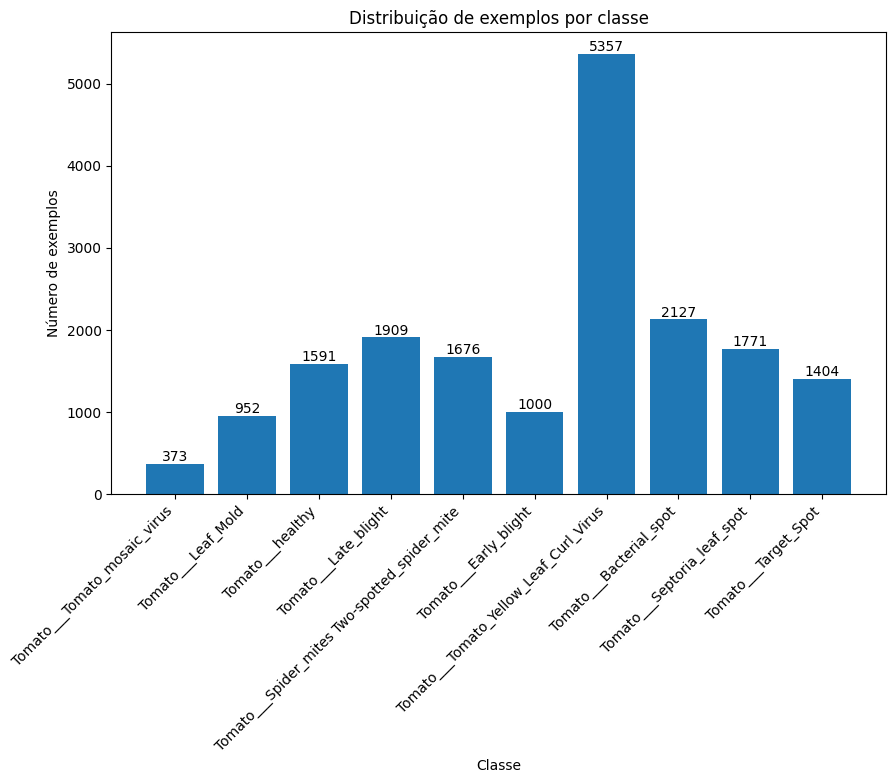
\includegraphics[width=0.9\linewidth]{images/plant_village_distribution.png}
    \caption{\label{fig:distribuicao_plantvillage} Distribuição de exemplos por classes de tomate no PlantVillage. Fonte: acervo dos autores.}
\end{figure}

Como o \emph{PlantVillage} possui uma única folha por imagem e é destinado à tarefa de classificação, a ideia para fazer essa integração é utilizar a área inteira das imagens do \emph{PlantVillage} como \emph{bounding box}.

\section{Busca de imagens por similaridade}
Como comentado anteriormente, é importante que um conjunto de dados robusto não tenha duplicatas ou ``quase-duplicatas'' em seus dados. No sistema atual, não há uma maneira de assegurar que somente imagens distintas farão parte do conjunto de dados resultante. Nesse sentido, para que os conjuntos de dados produzidos pelo \emph{TomatoHealth} não tenham dados repetidos, pensamos em um próximo passo que apresente as imagens mais semelhantes à que está sendo revisada. Assim, caso o usuário especialista interprete que ela é semelhante demais com imagens já presentes no conjunto de dados atual, será possível cancelar sua adição ao conjunto de dados atualizado.

Para fazer isso, pensamos no seguinte passo a passo:
\begin{enumerate}
    {\bf  \item Produzir representações em alto nível de cada imagem que faz parte do conjunto de dados:} essas representações, também conhecidas como \emph{embeddings}, não são nada mais que o resultado da extração de características de cada imagem. É mais simples e eficiente armazenar e comparar uma imagem com as demais se ela for representada como um vetor de 512 dimensões, por exemplo, ao invés de uma matriz de \emph{pixels} de $256 \times 256 \times 3$ dimensões.
    {\bf \item Armazenar esses \emph{embeddings} em um banco de dados de vetores:} podemos utilizar modelos de redes convolucionais pré-treinadas no \emph{dataset ImageNet}, boas em extração de características, para produzir os \emph{embeddings} de todas as imagens o conjunto de dados e então armazenar essas extrações em um banco de dados de vetores. Isso é importante pois, assim, só precisaremos obter essas representações uma única vez. Seguindo essa lógica, depois da revisão de toda imagem por um usuário especialista, devemos produzir sua representação vetorial e armazená-la no banco de dados vetorial.
    {\bf \item Fazer busca por similaridade no banco de dados vetorial:} no momento em que um usuário especialista for fazer a revisão de uma nova imagem, devemos fazer a busca por similaridade com as imagens presentes no banco de dados vetorial e, por conseguinte, no conjunto de dados. Isso é uma tarefa recorrente e há diversas ferramentas que disponibilizam esse serviço. Podemos comentar sobre a \emph{Pinecone}\footnote{\url{https://www.pinecone.io/learn/what-is-similarity-search/\#What-Are-Vector-Representations}}, que inclusive disponibiliza uma busca pelos $K$ vetores mais semelhantes ao examinado.
     {\bf \item Exibir as imagens mais semelhantes:} basta exibir as imagens mais semelhantes ao usuário especialista.
\end{enumerate}

\section{Mudança de \emph{LLM}}

Atualmente, como descrito no artigo, utilizamos uma chamada de \textit{API} a um modelo de linguagem (\texttt{gpt-4o-mini}) disponibilizado pela \textit{OpenAI} para gerar a resposta de diagnóstico ao usuário. No entanto, tal serviço é pago e adiciona dependências a serviços de terceiros ao projeto \emph{TomatoHealth}. Dessa forma, é interessante trabalhar para que essa funcionalidade seja incorporada de maneira mais natural ao projeto, sem implicar em custos monetários e que seja independente de terceiros. Isso pode ser feito com a adição um programa que rode um modelo de linguagem (\emph{LLM}) como um \emph{container} no ecossistema do \emph{Docker Compose}. Para isso, poderíamos utilizar a ferramenta \emph{HuggingFace Transformers}\footnote{\url{https://huggingface.co/docs/transformers/index}}, que torna simples o processo de inferência e treinamento de modelos de linguagem atuais.
